\documentclass[11pt,a4paper]{article}
\usepackage[T1]{fontenc}
\usepackage[utf8]{inputenc}
\usepackage{newtxtext,newtxmath,microtype}
\usepackage[margin=20mm,headheight=14pt]{geometry}
\usepackage{amsmath,booktabs,tabularx,array,caption,float,graphicx,siunitx,listings}
\usepackage{xcolor,fancyhdr,lastpage}
\usepackage[hidelinks]{hyperref}
\definecolor{accent}{HTML}{254C58}
\hypersetup{pdftitle={Section 3 -- Magnetoquasistatic analysis},pdfauthor={Tiebert Lefebure}}
\pagestyle{fancy}\fancyhf{}
\fancyhead[L]{\small Finite Elements for Electromagnetic Fields}
\fancyhead[R]{\small NKT 33 kV XLPE-AL}
\fancyfoot[L]{\small Section 3: Magnetoquasistatic analysis}
\fancyfoot[R]{\small \thepage\,/\,\pageref{LastPage}}
\setlength{\parindent}{0pt}\setlength{\parskip}{3pt}
\setlength{\intextsep}{5pt}
\AtBeginDocument{\fontsize{10.5}{12.6}\selectfont
 \setlength{\abovedisplayskip}{7pt}\setlength{\belowdisplayskip}{7pt}
 \setlength{\abovedisplayshortskip}{4pt}\setlength{\belowdisplayshortskip}{4pt}}
\setlength{\emergencystretch}{2em}
\renewcommand{\arraystretch}{1.15}\setlength{\tabcolsep}{5pt}
\captionsetup{font=small,labelfont=bf,skip=5pt}
\newcolumntype{Y}{>{\raggedright\arraybackslash}X}
\newcommand{\pagetitle}[2]{{\Large\bfseries #1}\par{\large #2}\par\medskip}
\newcommand{\subhead}[1]{\par\smallskip{\large\bfseries #1}\par\smallskip}
\newcommand{\val}[1]{\num[round-mode=places,round-precision=4]{#1}}
\newcommand{\rval}[1]{\num[round-mode=places,round-precision=6]{#1}}
\newcommand{\pct}[1]{\num[round-mode=places,round-precision=3]{#1}\%}
\lstdefinestyle{command}{basicstyle=\ttfamily\small,columns=fullflexible,keepspaces=true,
 backgroundcolor=\color{accent!5},aboveskip=4pt,belowskip=5pt,
 xleftmargin=5pt,xrightmargin=5pt,breaklines=true,showstringspaces=false}
\newcommand{\guidetitle}{\par\smallskip{\small\bfseries\color{accent}Code guide}\par}
\newcommand{\codeguide}[3]{%
 \begingroup\small\setlength{\tabcolsep}{0pt}\renewcommand{\arraystretch}{1}%
 \begin{tabularx}{\linewidth}{@{}p{20mm}Y@{}}
 \textbf{Computes} & #1\\[1pt]
 \textbf{Read} & #2\\[1pt]
 \textbf{Inspect} & #3
 \end{tabularx}\par\endgroup\smallskip}
\newcommand{\BaseLoss}{69.987740}
\newcommand{\BaseR}{0.135458}
\newcommand{\BaseL}{0.377822}
\newcommand{\BaseB}{11.620549}
\newcommand{\AlLoss}{65.200336}
\newcommand{\CuLoss}{4.787404}
\newcommand{\AlR}{0.126192}
\newcommand{\CuR}{0.009266}
\newcommand{\ExtraR}{0.001192}
\newcommand{\DeltaAl}{11.989029}
\newcommand{\DeltaCu}{9.227343}
\newcommand{\SkinR}{0.125655}
\newcommand{\AnalyticL}{0.385529}
\newcommand{\ProximityR}{0.000556}
\newcommand{\ScreenFeedbackR}{-0.000019}
\newcommand{\SingleLoss}{66.127811}
\newcommand{\SingleCu}{0.920430}
\newcommand{\Saving}{5.515150}
\newcommand{\SavingAbsolute}{3.859929}
\newcommand{\StrandedDifference}{0.714640}
\newcommand{\FineLossChange}{0.081159}
\newcommand{\FineLChange}{0.022387}
\newcommand{\SimplifiedLossChange}{0.000048}
\newcommand{\SimplifiedLChange}{0.006563}
\newcommand{\DatasheetLDifference}{-1.086365}
\newcommand{\AnalyticLDifference}{-0.092978}
\newcommand{\AnalyticLFE}{0.385171}
\newcommand{\DomainLChange}{0.138092}
\newcommand{\Quality}{0.056459}
\newcommand{\MetalQuality}{0.729828}
\newcommand{\AlEdge}{0.941048}
\newcommand{\CuEdge}{0.369412}

\newcommand{\DomainRows}{%
0.25 & 69.82853 & 0.375665 \\
0.5 & 69.98774 & 0.377822 \\
1 & 70.02688 & 0.378345 \\
}

\newcommand{\MeshRows}{%
2 & 3,138 & 70.5893 & 0.136622 & 0.376790 \\
1 & 9,624 & 70.2193 & 0.135906 & 0.377642 \\
0.5 & 29,984 & 69.9877 & 0.135458 & 0.377822 \\
0.25 & 106,528 & 69.9310 & 0.135348 & 0.377907 \\
}

\newcommand{\ComparisonRows}{%
Massive, solid bonding & 65.2003 & 4.7874 & 69.9877 & 0.37782 \\
Stranded, solid bonding & 64.6664 & 4.8247 & 69.4911 & 0.37869 \\
Massive, single point & 65.2074 & 0.9204 & 66.1278 & 0.38350 \\
Massive, inactive copper & 65.2100 & 0.0000 & 65.2100 & 0.38423 \\
Merged nonmetal layers & 65.2003 & 4.7875 & 69.9878 & 0.37785 \\
}

\newcommand{\LossRows}{%
Aluminium A & 21.73344 \\
Aluminium B & 21.73344 \\
Aluminium C & 21.73345 \\
Copper screen A & 1.59569 \\
Copper screen B & 1.59587 \\
Copper screen C & 1.59584 \\
Semiconducting regions & 1.513e-10 \\
Soil & 1.113e-07 \\
Armour / pipe & 0 (absent) \\
Total & 69.98774 \\
}

\newcommand{\CurrentRows}{%
Al A & 415.0000 & -0.00 & 2.0123 \\
Al B & 415.0000 & -120.00 & 2.0123 \\
Al C & 415.0000 & 120.00 & 2.0123 \\
Cu A & 62.1790 & -101.00 & 1.7577 \\
Cu B & 62.1825 & 139.00 & 1.7579 \\
Cu C & 62.1821 & 19.00 & 1.7579 \\
}

\newcommand{\FrequencyRows}{%
5 & 0.125266 & 0.384495 & 0.0501 \\
50 & 0.135458 & 0.377822 & 4.7874 \\
200 & 0.228673 & 0.321192 & 47.0489 \\
1000 & 0.496566 & 0.217398 & 136.1170 \\
}

% Original question wording: NMES Assignment 2026, Sections 1 and 2.
% Line-wrap hyphenation is removed; mathematical notation is typeset in LaTeX.
\usepackage{tcolorbox}
\newcommand{\assignmentquestion}[1]{%
  \begin{tcolorbox}[colback=accent!4,colframe=accent!65,
    boxrule=0pt,leftrule=2pt,arc=0pt,boxsep=0pt,
    left=7pt,right=7pt,top=5pt,bottom=5pt,
    before skip=0pt,after skip=8pt,fontupper=\small]
  \textbf{Assignment question.} #1
  \end{tcolorbox}%
}
\newcommand{\questionfiles}[1]{%
  \par\smallskip{\footnotesize\color{accent}
  \textbf{Files / results (relative to Source-code).} #1\par}\medskip
}
\newcommand{\QuestionOneOne}{%
Describe your cable: construction, dimensions, materials, rated voltage, rated
current (ampacity) and the laying conditions for which that rating is given
(burial depth, soil thermal resistivity, ambient temperature, arrangement).
Give a table of electromagnetic and thermal properties with a source for each value.}
\newcommand{\QuestionOneTwo}{%
Choose the environment consistently with the datasheet rating conditions,
and justify its properties.}
\newcommand{\QuestionOneThree}{%
State the sheath bonding you assume: single-point bonded (no net sheath current)
or solidly bonded (circulating sheath currents allowed), and how the armour
and pipe are connected. This choice strongly affects the losses in Section 3.}
\newcommand{\QuestionOneFour}{%
State the excitation you impose: phase-to-ground voltage and phase current,
as peak phasors, with the phase sequence (see the conventions in Appendix A).}
\newcommand{\QuestionTwoOne}{%
Define your computational domain, the equations solved and the boundary
conditions. Where do you truncate the domain, and why? Discuss the role of
the grounded screens: which regions actually influence the field in the insulation?}
\newcommand{\QuestionTwoTwo}{%
Can you simplify the geometry of your cable without degrading the precision
(e.g. disregard details in the geometrical description)? Quantify the effect
of each simplification.}
\newcommand{\QuestionTwoThree}{%
How do the results vary with the mesh refinement? Plot the maximum field in
the insulation and the capacitance versus the number of degrees of freedom,
and identify where local refinement is needed.}
\newcommand{\QuestionTwoFour}{%
Define the admissible field strength at the conductor screen and at the core
screen from the datasheet (or, if absent, from a cited reference).
Is the healthy cable within these limits?}
\newcommand{\QuestionTwoFive}{%
Add a defect to the insulation of your cable. State its nature (e.g. gas void,
water tree, protrusion of the semiconducting screen), its properties, size and
position, and discuss what a defect in a 2D cross-section represents in 3D.
Compare the field with and without defect along a radial cut.
Does the cable withstand the defect?}
\newcommand{\QuestionTwoSix}{%
Compute the resistive and displacement current densities in the cable.
Is current conservation satisfied? Which current dominates in each material, and why?}
\newcommand{\QuestionTwoSeven}{%
Compute the per-unit-length capacitance (\(\mu\mathrm{F/km}\)) and compare with
the analytical value (13) and with the datasheet. State the assumptions of the
analytical formula (in particular, how the semiconducting layers are treated).
Does the capacitance vary with frequency? Why (not)?}
\newcommand{\QuestionTwoEight}{%
Propose an improvement of the cable design with respect to the electric stress,
and support it quantitatively.}

\begin{document}

\pagetitle{Running Section 3}{Setup, commands and result files}
\subhead{Set up Python once}
From the repository root, create the environment, install the three required
packages, activate it and enter the Section 3 folder:
\begin{lstlisting}[style=command]
python3 -m venv .venv
.venv/bin/python -m pip install -r \
  Source-code/section_3/requirements.txt
source .venv/bin/activate
cd Source-code/section_3
\end{lstlisting}
The packages are NumPy, SciPy and Matplotlib. Gmsh and GetDP must also be installed.
The runner searches PATH and the neighbouring ONELAB installation; use
\texttt{--gmsh /path/to/gmsh} and \texttt{--getdp /path/to/getdp} to override them.
In a new terminal, activate the environment and enter the folder again.

\subhead{How to use the question guides}
All commands and paths in the guides below refer to \path{Source-code/section_3},
with the environment activated. Each guide identifies the cases, code and outputs
needed for its answer.

\texttt{python run.py --study} runs all 15 controlled cases, including mesh,
domain, conductor, bonding and frequency comparisons. \textbf{Run it once and reuse
the results for later guides that show the same command.} Rerun after changing model
inputs. A single-case command runs only the named case; \texttt{--open} also opens
its field maps in Gmsh.

\texttt{python report.py} reads the completed study and exports the report's
tables, figures, analytical checks and the baseline/single-point Gmsh viewers.
It performs no FE solve. Run it after the full study, before using the report's
comparison figures or analytical checks.

\begin{table}[H]\centering\small
\begin{tabularx}{\linewidth}{@{}p{55mm}Y@{}}\toprule
File or folder & What to use it for\\\midrule
\path{prepare.py} & Read Section 1 inputs and generate \path{parameters.inc}.\\
\path{model.geo}, \path{settings.inc} & Layers, physical tags, mesh and case switches.\\
\path{model.pro} & Magnetic equations, imposed currents and screen bonding.\\
\path{run.py}, \path{study.py} & Execute a named case or the full comparison study.\\
\path{analyse.py} & Calculate fields, currents, losses, energy and numerical checks.\\
\path{report.py} & Export checked tables, figures and analytical comparisons.\\
\path{results/<case>/view.geo} & Open in Gmsh; toggle magnetic, current and loss views.\\
\path{results/<case>/metrics.json} & Open in a text editor for one case's numerical results.\\
\path{validation/summary.json} & Same metrics, collected under the 15 case names.\\\bottomrule
\end{tabularx}\end{table}
In \path{metrics.json}, \texttt{regions} uses physical tags as keys:
Al A/B/C are \texttt{100/200/300}, copper A/B/C are \texttt{105/205/305},
and soil is \texttt{900}. Complex values are stored as \texttt{[real, imaginary]}
with peak amplitudes; divide their norms by \(\sqrt2\) for RMS values.
\path{fields.npz} contains arrays used by the plotting scripts; it need not be opened manually.

\newpage
\pagetitle{Magnetic model and excitation}{Q3.1 --- Domain, equations and boundary conditions}
\assignmentquestion{\QuestionThreeOne}
\guidetitle
\begin{lstlisting}[style=command]
python run.py --study
python report.py
\end{lstlisting}
\codeguide
 {The full study; for this answer compare \texttt{small\_domain}, \texttt{baseline}
  and \texttt{large\_domain}, with outer radii 0.25, 0.5 and 1 m.}
 {\path{model.geo} creates the cable/soil domain; \path{model.pro} defines
  \texttt{FarField}, \texttt{CurrentConstraint} and the magnetic weak form.}
 {\path{validation/summary.json}: compare \texttt{loss\_total\_W\_m} and
  \texttt{inductance\_mH\_km} in the three cases; \texttt{options/OuterRadius}
  records the truncation radius.}
The model is three NKT \(1\times240+50~\mathrm{mm^2}\) single-core cables,
touching in trefoil with centre spacing \(D=45.5~\mathrm{mm}\). It retains
the solid aluminium cores, semiconducting layers, XLPE, equal-area copper
screens, PE jackets and soil. There is no armour or pipe [1,2].
The trefoil centroid is the coordinate origin; its burial depth remains 1 m.
The magnetic problem uses a circular truncation of radius \(R_b=0.5~\mathrm m\).
All regions have \(\mu=\mu_0\). Constant metal conductivities are evaluated
at \(20^\circ\mathrm C\), with \(I=415~\mathrm A\) RMS and \(f=50~\mathrm{Hz}\).

With peak phasors and \(e^{\mathrm j\omega t}\), use
\[
 \widehat{\mathbf A}=\widehat a_z\mathbf e_z,\quad
 \widehat{\mathbf B}=\nabla\times\widehat{\mathbf A},\quad
 \nabla\times(\mu_0^{-1}\nabla\times\widehat{\mathbf A})=\widehat{\mathbf J},
 \qquad \widehat J_{z,m}=-\sigma_m(\mathrm j\omega\widehat a_z+g_m).
\]
Here \(g_m=\partial\widehat v/\partial z\) is one unknown constant per
massive region; the physical longitudinal voltage drop is \(u'_m=-g_m\).
The weak magnetic equation is
\[
 \int_\Omega\mu_0^{-1}\operatorname{curl}\widehat{\mathbf A}\cdot
 \operatorname{curl}\mathbf w\,dA
 +\int_{\Omega_C}\sigma(\mathrm j\omega\widehat{\mathbf A}+g\mathbf e_z)
 \cdot\mathbf w\,dA=\int_{\Omega_S}\widehat{\mathbf J}_s\cdot\mathbf w\,dA.
\]
One integral-current equation closes each current-driven region. The default
has \(\Omega_S=\varnothing\); stranded phases are an explicit comparison case.

\subhead{Currents and interfaces}
For A, B, C, impose the net phase currents, rather than a local current density:
\[
 \int_{\Omega_k}\widehat J_z\,dA=\widehat I_k,
 \qquad \widehat I_k=\sqrt2(415)e^{-\mathrm j2\pi k/3}~\mathrm A,
 \quad k=0,1,2.
\]
The peak amplitude is \(586.8986~\mathrm A\). Shared interface nodes enforce
continuity of \(a_z\); the weak form supplies tangential \(H\) continuity.
At the outer circle impose \(a_z=0\), representing the distant return reference.
The balanced system has no net applied phase current and a decaying far field.

\begin{table}[H]\centering\small
\caption{Boundary sensitivity at fixed local mesh sizes.}
\begin{tabular}{@{}rrr@{}}\toprule
\(R_b\) [m] & Total loss [kW/km] & \(L\) [mH/km]\\\midrule
\DomainRows\bottomrule\end{tabular}
\end{table}
Doubling the selected radius changes \(L\) by \pct{\DomainLChange}.
The soil uses \(\sigma=0.01~\mathrm{S/m}\) and no applied axial voltage
gradient. The ground/air interface is omitted: both have \(\mu_r\simeq1\),
and a separate zero-soil-conductivity solve checks its negligible magnetic influence.

\newpage
\pagetitle{Massive or stranded conductors}{Q3.2 --- Skin depth and the conductor model}
\assignmentquestion{\QuestionThreeTwo}
\guidetitle
\begin{lstlisting}[style=command]
python run.py --study
python report.py
\end{lstlisting}
\codeguide
 {Compares \texttt{baseline} (massive phases) with \texttt{stranded} (uniform phase current).
  The study also supplies the other rows in the comparison table.}
 {\texttt{Stranded} in \path{model.pro} switches between imposed net current and
  uniform current density. \path{analyse.py} calculates skin depths and integrated losses.}
 {In \path{validation/summary.json}, compare the two cases' conductor/screen losses and
  \texttt{inductance\_mH\_km}. \texttt{mesh/aluminium/skin\_depth\_mm} gives \(\delta_{\rm Al}\).}
For a nonmagnetic metal,
\[
 \delta=\sqrt{\frac{2}{\omega\mu_0\sigma}},\qquad
 \delta_{\rm Al}=\val{\DeltaAl}~\mathrm{mm},\quad
 \delta_{\rm Cu}=\val{\DeltaCu}~\mathrm{mm}\qquad (50~\mathrm{Hz}).
\]
The aluminium radius is \(8.5~\mathrm{mm}\), so \(r/\delta_{\rm Al}=0.709\).
Skin effect is moderate rather than severe. The copper screen thickness is
\(0.39887~\mathrm{mm}\), only \(0.0432\delta_{\rm Cu}\); its radial skin
effect is weak, but its net circulating current and azimuthal redistribution
still dissipate power.

\subhead{Two implemented models}
\textbf{Stranded.} Set \(\widehat J_{z,k}=\widehat I_k/A_{k,h}\), uniform
over each meshed conductor area \(A_{k,h}\). Normalising by the mesh area
preserves the exact imposed net current despite the polygonal circle boundary.
There is no skin or proximity redistribution inside the phase. Its terminal
drop follows from the uniform-current resistive drop and the cross-sectional
mean of \(\mathrm j\omega a_z\).

\textbf{Massive.} Solve \(a_z\) and \(g_k\), imposing only
\(\int\widehat J_z\,dA=\widehat I_k\). The local distribution is free to
respond to self and neighbouring magnetic fields. This includes both skin
and proximity effects. The copper remains massive in both comparisons.

\begin{table}[H]\centering\small
\caption{Controlled comparisons at 415 A RMS, 50 Hz and constant conductivity.}
\begin{tabularx}{\linewidth}{@{}Yrrrr@{}}\toprule
Model & Al loss & Cu loss & Total & \(L\)\\
 & \multicolumn{3}{c}{[kW/km]} & [mH/km]\\\midrule
\ComparisonRows\bottomrule\end{tabularx}
\end{table}
The massive model raises total loss by \pct{\StrandedDifference} relative to
the uniform-current model. It also changes the field, induced screen current
and inductance slightly; these quantities cannot be corrected by adding a
skin-loss number after the solve.

\subhead{Choice for the selected cable}
The NKT construction explicitly states a \emph{circular solid aluminium
conductor} [2]. The massive model therefore represents the cable more closely.
A stranded approximation is useful for comparison, but a nominal cable area
does not imply insulated strands or suppressed eddy currents.

The geometric aluminium area is \(226.980~\mathrm{mm^2}\), while the product
designation is 240 \(\mathrm{mm^2}\). Following Section 1, use the effective
conductivity \(3.52454\times10^7~\mathrm{S/m}\), calibrated to the maximum
datasheet DC resistance. The diameter, nominal designation and calibrated
conductivity are not three independent measurements of the metal.

\newpage
\pagetitle{Screen bonding as a circuit condition}{Q3.3 --- Global currents and voltage drops}
\assignmentquestion{\QuestionThreeThree}
\guidetitle
\begin{lstlisting}[style=command]
python run.py --case baseline
python run.py --case single_point --single-point
\end{lstlisting}
\codeguide
 {The same cable with both-end and single-point screen bonding.}
 {In \path{model.pro}, follow \texttt{SinglePoint} through \texttt{CurrentConstraint},
  \texttt{GradientConstraint}, the \texttt{Gradient} space and \texttt{GlobalTerm}.}
 {Each case's \path{metrics.json}: under \texttt{regions}, copper tags
  \texttt{105/205/305} contain \texttt{current\_peak\_A} and
  \texttt{voltage\_drop\_peak\_V\_m}. Check zero voltage drop for both-end bonding,
  versus zero net screen current for single-point bonding.}
Section 1 selected copper screens bonded to common earth at both ends, with
ideal bonding leads and no cross-bonding. For each copper screen \(s\),
\[
 u'_s=-g_s=0,\qquad
 \widehat I_s=\int_{\Omega_s}-\sigma_s(\mathrm j\omega\widehat a_z+g_s)\,dA
 \quad\text{is a result.}
\]
The screens are separate massive regions, not a shared equipotential magnetic
boundary. There are no armour or pipe quantities because those components
are absent. Bonding lead resistance, end-earth impedance and helical lay are
outside the present 2D model.

\subhead{Implementation}
The region basis \texttt{BF\_RegionZ} supplies one longitudinal gradient
coefficient per massive region. \texttt{G} is its \texttt{AliasOf} global
quantity; \texttt{I} is the energy-dual \texttt{AssociatedWith} quantity [3,4].
For a current-driven region, the additional equation is
\[
 \int_{\Omega_m}\sigma_m(\mathrm j\omega\widehat a_z+g_m)\,dA
 +\widehat I_m=0.
\]
For a voltage-driven screen, the gradient coefficient is assigned zero and
the current is recovered by integrating the complete \(J_z\). This makes
the change to single-point bonding explicit:
\[
 \text{single point:}\qquad \widehat I_s=0,\quad g_s\ \text{unknown}.
\]
The semiconductor regions are assigned zero net axial current as an auxiliary
closure; their extremely small conductivity makes their contribution negligible.
Their actual axial end connections are not specified by the datasheet.

\subhead{Why the \(a_z\)-only expression is insufficient}
Writing \(\widehat J_z=-\mathrm j\omega\sigma\widehat a_z\) alone silently
sets \(g=0\), without stating the external voltage or current constraint.
It cannot express an isolated screen with zero net current. Moreover, under
\(a_z\mapsto a_z+C\), the same physical electric field requires
\(g\mapsto g-\mathrm j\omega C\). Dropping \(g\) without fixing a return
reference can therefore make the inferred current depend on the potential
reference. Here \(a_z=0\) at the far boundary and \(u'_s=0\) are both stated:
the reduced expression then follows from the selected solid-bonding condition.

\subhead{Numerical consequence}
Solid bonding gives \val{\CuLoss} kW/km in copper. Single-point bonding
reduces that to \val{\SingleCu} kW/km; it does not eliminate local eddy
currents. Total loss falls from \val{\BaseLoss} to \val{\SingleLoss} kW/km.
This difference is a circuit-condition effect, with identical cable dimensions.

\newpage
\pagetitle{Geometry simplifications}{Q3.4 --- What can be removed from the magnetic model?}
\assignmentquestion{\QuestionThreeFour}
\guidetitle
\begin{lstlisting}[style=command]
python run.py --study
python report.py
\end{lstlisting}
\codeguide
 {The full study; focus on \texttt{baseline}, \texttt{simplified},
  \texttt{no\_screens} and \texttt{no\_soil}.}
 {\texttt{Detailed} in \path{model.geo} merges the nonmetal layers.
  \texttt{Screens} in \path{model.pro} controls copper conductivity;
  \path{study.py} selects each comparison's settings.}
 {\path{validation/summary.json}: compare \texttt{loss\_total\_W\_m} and
  \texttt{inductance\_mH\_km} with \texttt{baseline}.
  Read \texttt{options} to check which assumption changed.}
\textbf{The Section 2 truncation is not valid here.} Grounded copper screens
confine the transverse electric field but do not confine the magnetic field.
The phase interiors, metallic screens and surrounding magnetic space must
remain in the MQS problem. Treating every grounded screen as \(a_z=0\)
would impose an artificial magnetic shield and suppress the physical coupling.

\subhead{Quantified changes}
\begin{table}[H]\centering\small
\caption{Simplifications and their interpretation.}
\begin{tabularx}{\linewidth}{@{}p{43mm}Y@{}}\toprule
Change & Finding / decision\\\midrule
Merge inner SC, XLPE, outer SC and contact bedding into one nonmagnetic,
nonconducting annulus & The actual internal interfaces are removed in the
\texttt{simplified} mesh. Total loss changes by less than 0.001\%
and inductance by \pct{\SimplifiedLChange}. The remaining difference also
includes the changed triangulation; SC losses themselves are negligible.\\
Suppress soil conductivity & The \texttt{no\_soil} case checks this directly.
The baseline soil loss is of order \(10^{-7}\) kW/km. Soil permeability and
the exterior domain must still be retained.\\
Deactivate copper conductivity & The \texttt{no\_screens} case retains its
geometry but makes it electromagnetically inactive. Loss and inductance
change visibly (Q3.2); copper cannot be discarded in the solid-bonded model.\\
Use uniform phase current & Total loss differs by \pct{\StrandedDifference}.
This approximation suppresses skin/proximity effects and is unnecessary for
the actual solid conductor.\\\bottomrule
\end{tabularx}\end{table}

\subhead{Equal-area copper annulus}
The real screen is copper wires with a counter-wound tape [2]. Its wire count,
wire diameter and lay lengths are not supplied. The model uses a continuous
annulus with outer radius 20.15 mm and metal area 50 \(\mathrm{mm^2}\), giving
inner radius 19.75113 mm. This preserves axial DC conductance for straight
copper but permits circumferential redistribution that a real wire/tape screen
may restrict. The annulus error cannot be established from the available data;
the mesh study verifies the equivalent model, not the undisclosed construction.

All zero-conductivity, nonmagnetic layers can be merged magnetically once
metal boundaries are preserved. The jackets remain explicit here to distinguish
the conducting soil. The small soil pocket between the touching jackets is
meshed as a separate surface sharing the jacket arcs. Omitting it leaves an
unphysical internal boundary and distorts both the field and inductance.

\newpage
\pagetitle{Mesh quality and convergence}{Q3.5 --- Resolve current redistribution and thin screens}
\assignmentquestion{\QuestionThreeFive}
\guidetitle
\begin{lstlisting}[style=command]
python run.py --study
python report.py
\end{lstlisting}
\codeguide
 {Four meshes: \texttt{coarse}, \texttt{medium}, \texttt{baseline} and \texttt{fine},
  with \texttt{MeshScale} 2, 1, 0.5 and 0.25.}
 {\path{study.py} sets the scales; \path{model.geo} sets local element sizes.
  \texttt{triangle\_geometry()} in \path{analyse.py} calculates element quality.}
 {\path{validation/summary.json}: compare DOFs, loss, resistance and inductance.
  Each case's \texttt{mesh} gives edge/skin-depth ratios; \texttt{min\_quality}
  and \texttt{conducting\_min\_quality} give the quality checks.}
First-order conforming triangles discretise \(a_z\). Four meshes are solved
with the same material and circuit data. The selected mesh has 29,984 complex
unknowns (59,968 real unknowns in this GetDP build); the finest has 106,528.
\begin{table}[H]\centering\small
\caption{Mesh convergence at fixed 0.5 m truncation radius.}
\begin{tabular}{@{}rrrrr@{}}\toprule
Scale & Complex DOFs & Loss [kW/km] & \(R\) [\(\Omega/\mathrm{km}\)] & \(L\) [mH/km]\\\midrule
\MeshRows\bottomrule\end{tabular}\end{table}
{\centering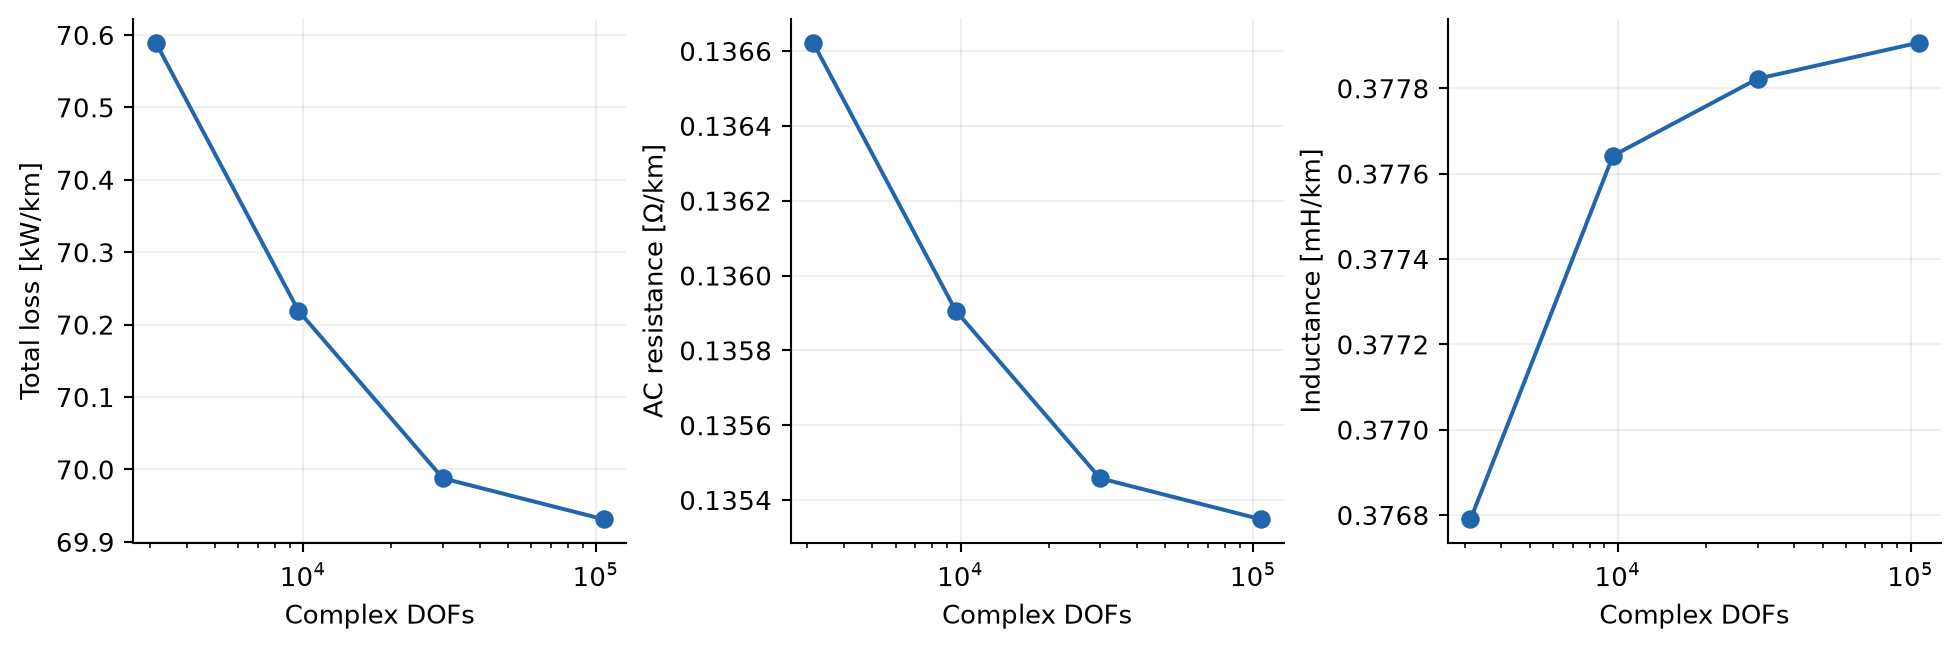
\includegraphics[width=\linewidth,height=4cm,keepaspectratio]{figures/convergence.png}\par}
Halving the selected mesh sizes changes loss and resistance by
\pct{\FineLossChange}, and inductance by \pct{\FineLChange}. A 0.5\% criterion
is satisfied for all three quantities. Domain-size error is checked separately
in Q3.1 rather than being attributed to mesh refinement.

The maximum aluminium edge is \val{\AlEdge} mm, below \(0.08\delta_{\rm Al}\).
In copper it is \val{\CuEdge} mm, below \(0.04\delta_{\rm Cu}\). Refinement
is driven by the thin screen and its azimuthal current variation, not only by
skin depth. Soil has \(\delta\simeq712~\mathrm m\) and needs no skin mesh.
At 1 kHz the study uses the finest mesh; the metal skin depths are smaller by
\(\sqrt{20}\) and remain resolved.

{\centering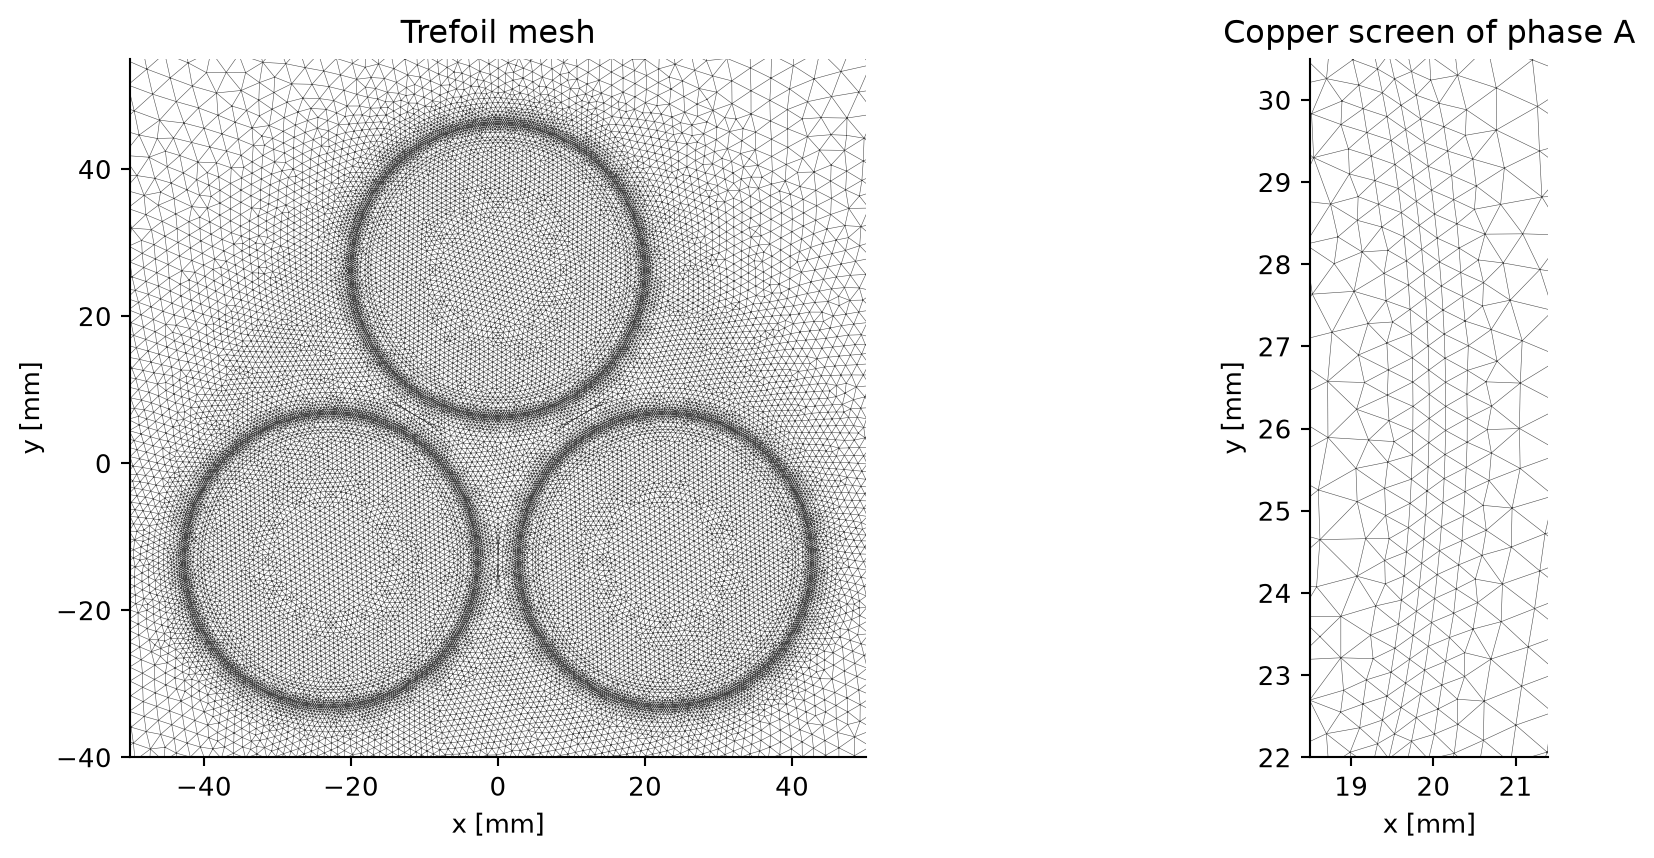
\includegraphics[width=0.94\linewidth,height=4.2cm,keepaspectratio]{figures/mesh.png}\par}
The triangle quality \(q=4\sqrt3 A/\sum_i\ell_i^2\) is 1 for an equilateral
triangle. Minimum \(q\) is \val{\Quality} overall and \val{\MetalQuality}
in conducting cable regions. The lowest-quality elements occur in the soil
cusps at jacket contacts. Every interior edge is checked for two incident
triangles; imposed currents and complex-power balance are checked after each solve.

\newpage
\pagetitle{Magnetic flux density}{Q3.6 --- Field in and around the trefoil}
\assignmentquestion{\QuestionThreeSix}
\guidetitle
\begin{lstlisting}[style=command]
python run.py --case baseline --open
\end{lstlisting}
\codeguide
 {The baseline magnetic field at 415 A RMS and 50 Hz.}
 {\texttt{analyse()} in \path{analyse.py} takes the curl of the P1 potential;
  \texttt{write\_views()} exports the RMS magnetic map.}
 {\path{results/baseline/view.geo}: show \texttt{RMS vector norm B [mT]}.
  In \path{results/baseline/metrics.json}, divide \texttt{max\_B\_phasor\_mT}
  by \(\sqrt2\) to reproduce the reported largest RMS norm.}
The magnetic flux density is recovered without smoothing from each element:
\[
 \widehat B_x=\frac{\partial\widehat a_z}{\partial y},\qquad
 \widehat B_y=-\frac{\partial\widehat a_z}{\partial x},\qquad
 B_{\rm rms,vec}=\sqrt{\frac{|\widehat B_x|^2+|\widehat B_y|^2}{2}}.
\]
The norm shown is the root mean square of the physical vector magnitude.
For an elliptically rotating field, the phasor vector norm divided by
\(\sqrt2\) is not the maximum instantaneous magnitude. This distinction
avoids interpreting complex-vector norms as a single real snapshot.

\begin{figure}[H]\centering
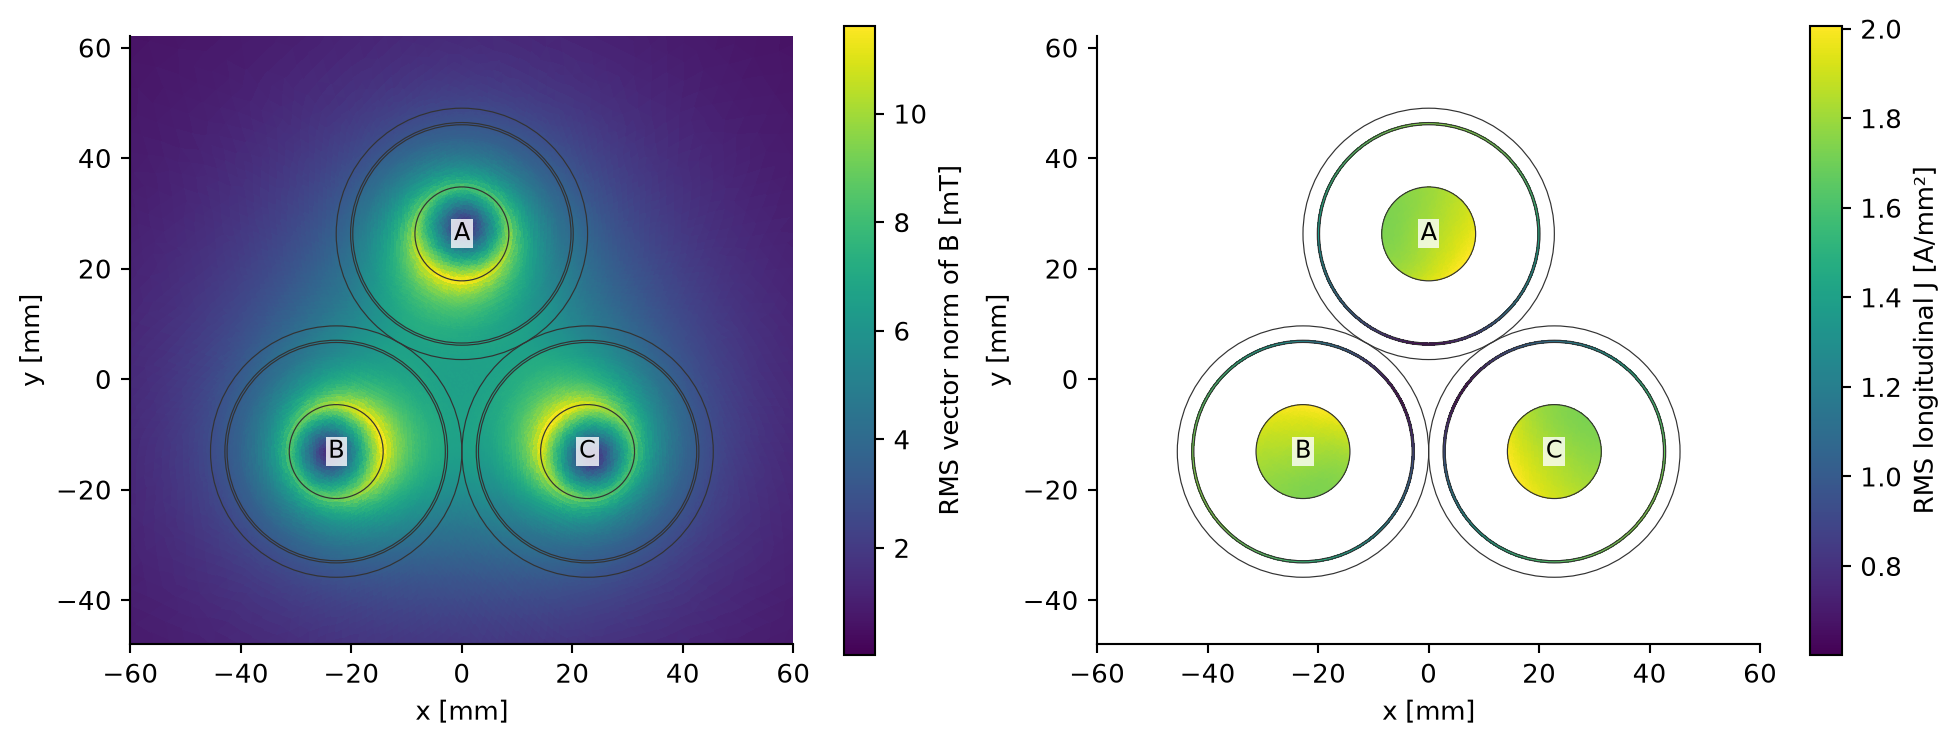
\includegraphics[width=\linewidth,height=5.8cm,keepaspectratio]{figures/baseline_fields.png}
\caption{Left: RMS vector norm of flux density in the cable region and nearby
soil. Right: RMS longitudinal current density, included for comparison.}
\end{figure}
The largest elementwise RMS flux-density norm is \val{\BaseB} mT.
The field is strongest near the phase conductors and is reshaped by the
induced copper currents. It extends through the grounded screens into the
soil. The balanced trefoil cancels the leading far-field contribution, so
the distant field falls more quickly than the field of one isolated wire.

\begin{figure}[H]\centering
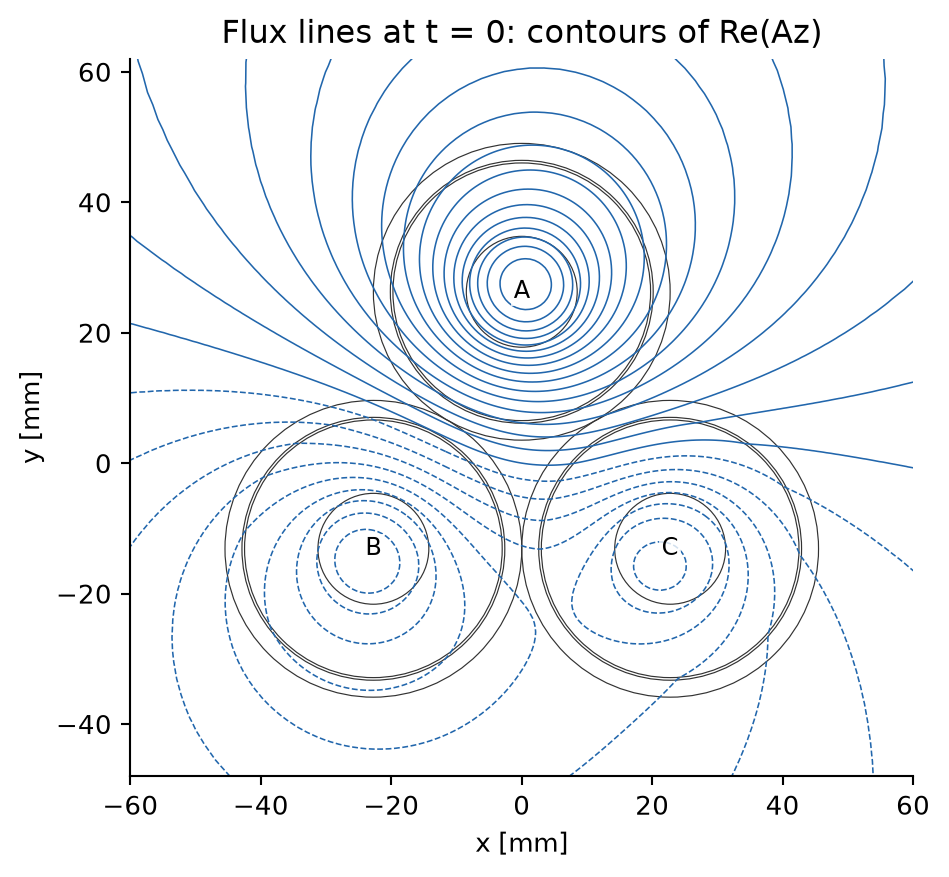
\includegraphics[width=0.72\linewidth,height=4.5cm,keepaspectratio]{figures/flux_lines.png}
\caption{Flux lines at \(t=0\): contours of \(\Re\{\widehat a_z\}\).
Phase A carries positive peak current.}
\end{figure}
With \(\mu_r=1\), conductivity changes affect eddy currents while normal \(B\)
remains continuous. Elementwise jumps come from P1 gradients; saturation and
hysteresis are not modelled.

\newpage
\pagetitle{Current density and net currents}{Q3.7 --- Redistribution in aluminium and copper}
\assignmentquestion{\QuestionThreeSeven}
\guidetitle
\begin{lstlisting}[style=command]
python run.py --case baseline --open
python run.py --case single_point --single-point
\end{lstlisting}
\codeguide
 {Baseline and single-point currents, using the same geometry and phase excitation.}
 {\texttt{analyse()} in \path{analyse.py} reconstructs \(J_z\) using both \(a_z\)
  and the regional gradient, then integrates the net current.}
 {In \path{results/baseline/view.geo}, show \texttt{RMS Jz [A/mm2]}.
  In each case's \path{metrics.json}, \texttt{regions/<tag>} contains
  \texttt{current\_peak\_A} and \texttt{max\_J\_peak\_A\_mm2}; divide peak norms by \(\sqrt2\).
  Copper tags are \texttt{105/205/305}.}
Use \(\widehat J_z=-\sigma(\mathrm j\omega\widehat a_z+g)\) in all massive
regions. The RMS scalar magnitude is \(|\widehat J_z|/\sqrt2\).
The aluminium current is mostly uniform, with moderate crowding from skin
and proximity effects. The screen current varies around the circumference,
despite the small ratio of screen thickness to copper skin depth.

\begin{table}[H]\centering
\caption{Baseline currents. Phase angles use the peak-phasor convention;
the final column is the largest nodal RMS current density.}
\begin{tabular}{@{}lrrr@{}}\toprule
Region & Net current [A RMS] & Angle [deg] & \(J_{\rm rms,max}\) [A/mm\(^2\)]\\\midrule
\CurrentRows\bottomrule\end{tabular}\end{table}
The phase currents integrate to 415 A RMS, with phases \(0^\circ,-120^\circ,+120^\circ\).
The three screen currents form an approximately balanced induced set. Their
phasors oppose part of the applied magnetic flux. A grounded screen therefore
does not have zero current, and its current is not generally in phase with
the current in the enclosed conductor.

\begin{figure}[H]\centering
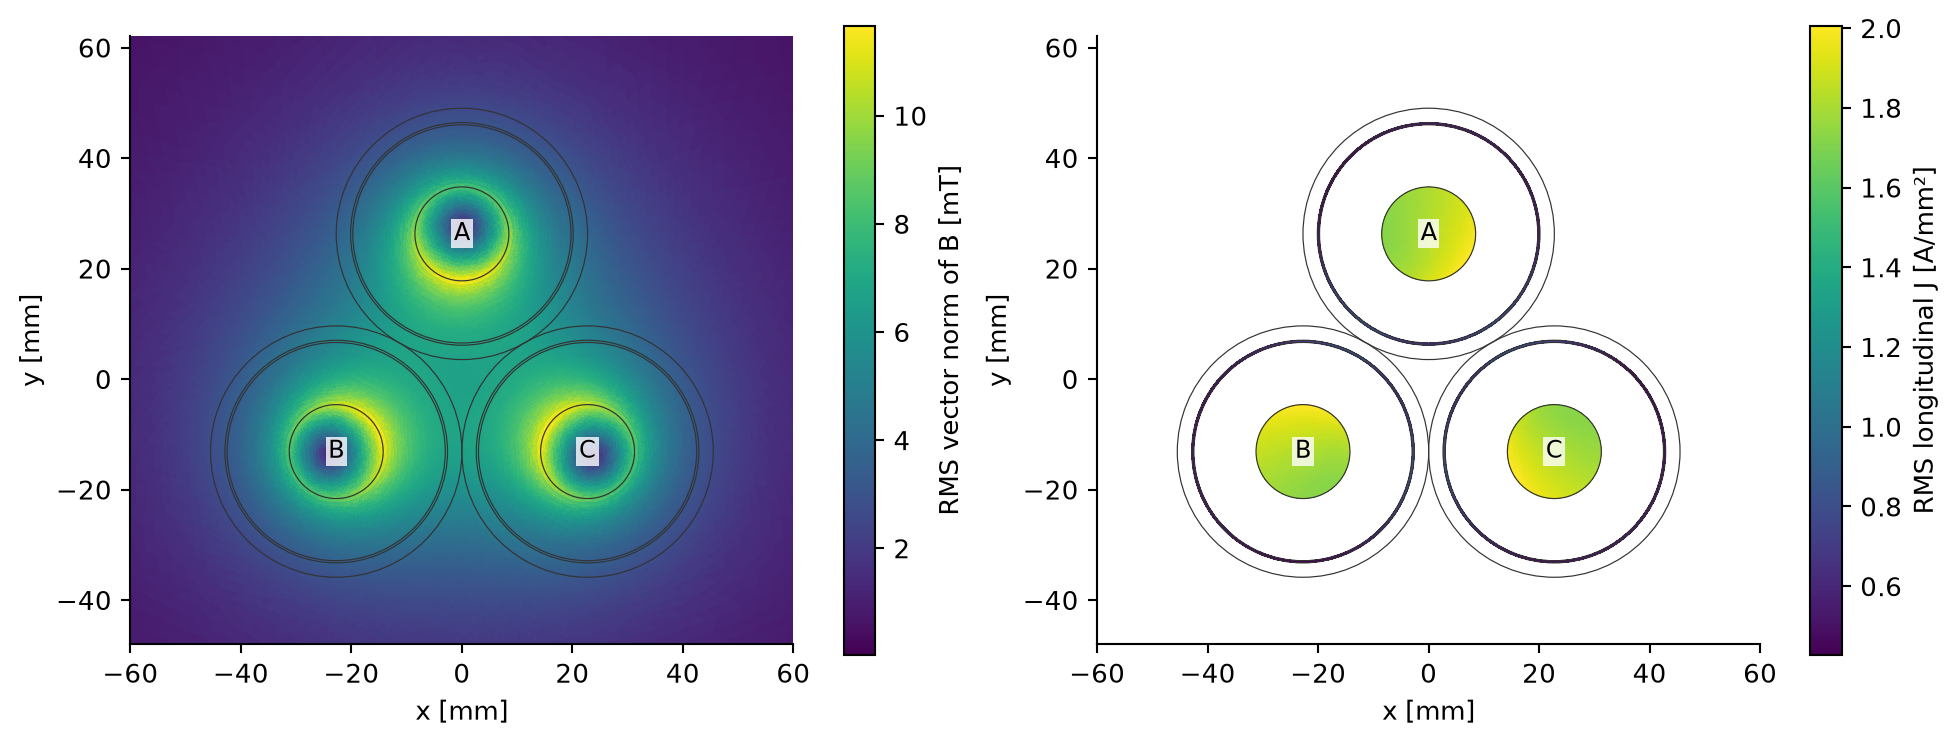
\includegraphics[width=\linewidth,height=5.8cm,keepaspectratio]{figures/single_point_fields.png}
\caption{The same geometry with single-point bonding. The copper screen has
zero integrated current, but nonzero local eddy current remains. Compare the
numerical colour scales with Q3.6; each map uses its own range.}
\end{figure}
At each solve, numerical integration checks the three imposed currents.
For zero-net-current regions it checks cancellation of positive and negative
longitudinal contributions rather than forcing the local current density to
vanish. Nonconducting XLPE and PE have zero MQS current; their transverse
charging currents belong to Section 2. Soil carries only the very small induced
axial current of this model. There is no injected earth-fault or neutral current.

\newpage
\pagetitle{Time-averaged Joule losses}{Q3.8 --- Losses in every conducting part}
\assignmentquestion{\QuestionThreeEight}
\guidetitle
\begin{lstlisting}[style=command]
python run.py --case baseline --open
\end{lstlisting}
\codeguide
 {The baseline loss density and integrated loss in each conducting region.}
 {\texttt{norm\_integral} in \path{analyse.py} integrates the squared P1 current
  exactly; \texttt{write\_views()} exports the loss-density map.}
 {In \path{results/baseline/view.geo}, show \texttt{Average Joule loss [W/m3]}.
  \path{results/baseline/metrics.json} gives \texttt{regions/<tag>/loss\_W\_m}
  and \texttt{loss\_total\_W\_m}. Numerically, W/m equals kW/km.}
For peak phasors the loss density and integrated loss are
\[
 \overline p_m=\frac{|\widehat J_z|^2}{2\sigma_m}
 =\frac{\sigma_m}{2}|\mathrm j\omega\widehat a_z+g_m|^2,\qquad
 P'_m=\int_{\Omega_m}\overline p_m\,dA.
\]
In particular, the phase loss must include \(g_m\). Computing only
\(\sigma\omega^2|a_z|^2/2\) would omit the imposed-current contribution
and would give the wrong heat source for Section 4. The supplied TA file is
retained as a reference; its massive-region \texttt{JouleLosses} expression
is replaced by the complete-current calculation here [3].

\begin{table}[H]\centering
\caption{Baseline losses at 415 A RMS, 50 Hz, constant \(20^\circ\mathrm C\)
conductivities. Numerically, 1 W/m = 1 kW/km.}
\begin{tabular}{@{}lr@{}}\toprule
Component & Time-averaged loss [kW/km]\\\midrule
\LossRows\bottomrule\end{tabular}\end{table}
Aluminium contributes \val{\AlLoss} kW/km and copper contributes
\val{\CuLoss} kW/km. The PE jacket is the nonmetallic outer sheath and has
no MQS conduction loss. The metallic sheath/screen loss is the copper entry.
No fictitious armour or pipe loss is added. Semiconductor losses are negligible
at the adopted \(0.002~\mathrm{S/m}\); soil losses are negligible too.

\subhead{Integration and energy checks}
The exported P1 potential makes \(J_z\) linear within each triangle. Its
squared norm is integrated with the exact triangle mass matrix, rather than
sampling only the centroid. For nodal complex currents \(J_1,J_2,J_3\),
\[
 \int_T|J_z|^2dA=\frac{A_T}{12}
 \left(\sum_{i=1}^3|J_i|^2+\left|\sum_{i=1}^3J_i\right|^2\right).
\]
An independent terminal check uses
\(\Re\{\frac12\sum_k u'_k\widehat I_k^*\}=\sum_mP'_m\).
The study also checks reactive power against magnetic energy. Full residuals
are recorded in \path{section_3/validation/RESULTS.md}.

These are linear, isothermal magnetic losses. They are not losses at the
90\(^{\circ}\)C operating limit, and they do not establish the cable ampacity.
Temperature-dependent metal conductivity and dielectric heat belong in Section 4.

\newpage
\pagetitle{AC resistance and loss separation}{Q3.9 --- A per-phase equivalent based on total loss}
\assignmentquestion{\QuestionThreeNine}
\guidetitle
\begin{lstlisting}[style=command]
python run.py --study
python report.py
\end{lstlisting}
\codeguide
 {The full study, including \texttt{baseline} and \texttt{no\_screens}, plus the
  isolated round-conductor reference used to separate the losses.}
 {\path{analyse.py} calculates total-loss resistance; \texttt{export()} in
  \path{report.py} calculates the skin, proximity and screen contributions.}
 {\texttt{resistance\_ohm\_km} in \path{results/baseline/metrics.json} is the total equivalent.
  The breakdown is in \path{validation/analytical_checks.json}, under \texttt{generated\_values}
  (\texttt{AlR}, \texttt{CuR}, \texttt{SkinR}, \texttt{ProximityR}, \texttt{ScreenFeedbackR}).}
Following the assignment, define the equivalent balanced-system resistance as
\[
 R'_{\rm AC,eq}=\frac{P'_{\rm total}}{3I_{\rm rms}^2},\qquad
 R_{\rm AC,eq}=1000R'_{\rm AC,eq}=\val{\BaseR}~\Omega/\mathrm{km}.
\]
It includes both phase-conductor and screen losses. It is not simply the
resistance of an isolated aluminium core. The NKT datasheet gives only the
maximum \emph{DC} core resistance, \(R_{\rm DC,20}=0.125~\Omega/\mathrm{km}\),
and does not publish an AC-resistance value for direct comparison [2].

\begin{table}[H]\centering
\caption{Resistance contributions for the baseline system.}
\begin{tabular}{@{}lr@{}}\toprule
Contribution & Equivalent resistance [\(\Omega/\mathrm{km}\)]\\\midrule
Calibrated aluminium DC reference & 0.125000\\
Aluminium skin/proximity increment & \rval{\ExtraR}\\
Total aluminium contribution & \rval{\AlR}\\
Copper-screen contribution & \rval{\CuR}\\
Total system equivalent & \rval{\BaseR}\\\bottomrule\end{tabular}\end{table}
The baseline exceeds the datasheet DC reference because the conductor current
is nonuniform and the screens dissipate power. A small additional difference
comes from approximating circular interfaces by straight mesh edges; refinement
reduces that area error.

\subhead{Separating self skin effect from proximity}
For an isolated round solid conductor, the cylindrical diffusion solution gives
\[
 Z'_{\rm int}=\frac{\kappa}{2\pi r\sigma}
 \frac{J_0(\kappa r)}{J_1(\kappa r)},\qquad
 \kappa=\frac{1-\mathrm j}{\delta}.
\]
Its real part is \(R_{\rm skin}=\rval{\SkinR}~\Omega/\mathrm{km}\),
only slightly above DC. With screen conductivity disabled, the FE aluminium
resistance exceeds this isolated-wire value by
\(\rval{\ProximityR}~\Omega/\mathrm{km}\). This residual is the neighbouring-phase
proximity contribution plus the small remaining mesh/domain error.

Restoring screen conductivity changes the aluminium contribution by
\(\rval{\ScreenFeedbackR}~\Omega/\mathrm{km}\), because the induced screen field
also changes core current crowding. Finally add the actual screen dissipation,
\(\val{\CuR}~\Omega/\mathrm{km}\). This controlled separation avoids counting
the screen-induced change in core loss as a second copper loss.

The semiconductor and soil contributions are below the displayed precision.
Armour contributes zero because it is absent. Calibration to the maximum
datasheet DC resistance is a modelling input, so agreement with that DC value
is not independent experimental validation.

\newpage
\pagetitle{Inductance of the three-phase system}{Q3.10 --- Balanced excitation, energy and frequency}
\assignmentquestion{\QuestionThreeTen}
\guidetitle
\begin{lstlisting}[style=command]
python run.py --study
python report.py
\end{lstlisting}
\codeguide
 {5, 50, 200 and 1\,000 Hz cases, plus \texttt{analytical\_trefoil} for the independent reference.}
 {\path{analyse.py} calculates magnetic energy and complex terminal power;
  \path{study.py} sets frequencies and refines the 1 kHz mesh.}
 {\path{validation/summary.json}: compare \texttt{inductance\_mH\_km} in
  \texttt{frequency\_5}, \texttt{baseline}, \texttt{frequency\_200} and \texttt{frequency\_1000}.
  \texttt{reactive\_balance\_relative} checks agreement between power and energy.}
For a balanced positive-sequence set, calculate equivalent per-phase
inductance from total time-averaged magnetic energy or terminal reactive power:
\[
 \begin{aligned}
 \overline W'_m&=\frac{1}{4\mu_0}\int_\Omega|\widehat{\mathbf B}|^2dA,
 & L'_{\rm eq}&=\frac{2\overline W'_m}{3I_{\rm rms}^2},\\[3pt]
 S'&=\tfrac12\sum_k u'_k\widehat I_k^*,
 & L'_{\rm eq}&=\frac{\Im S'}{3\omega I_{\rm rms}^2}.
 \end{aligned}
\]
The definitions agree numerically. This is the positive-sequence per-phase
equivalent including induced screen currents. Unbalanced excitation requires
an impedance matrix with mutual terms and a stated return path.

\textbf{Result:} \(L_{\rm eq}=\val{\BaseL}~\mathrm{mH/km}\).
NKT gives \(X=0.12~\Omega/\mathrm{km}\) at 50 Hz for touching trefoil [2], hence
\[
 L_{\rm NKT}=\frac{0.12}{2\pi50}~\mathrm{H/km}
 =0.381972~\mathrm{mH/km}.
\]
The signed FE difference is \pct{\DatasheetLDifference}. The datasheet value
is rounded to 0.01 \(\Omega/\mathrm{km}\), and its detailed screen/lay model
is unspecified; the comparison supports consistency, not sub-percent validation.

\subhead{Analytical and frequency checks}
For uniform phase currents without conducting screens, the equilateral-trefoil
estimate, including internal inductance, is
\[
 L_{\rm trefoil}\simeq0.2\left[\ln(D/r)+\frac14\right]
 =\val{\AnalyticL}~\mathrm{mH/km}.
\]
The matching FE case at \(R_b=1~\mathrm m\) gives \val{\AnalyticLFE} mH/km,
a signed difference of \pct{\AnalyticLDifference}. This checks the field
normalisation and three-phase energy factor independently of the NKT comparison.

\begin{table}[H]\centering\small
\begin{tabular}{@{}rrrr@{}}\toprule
\(f\) [Hz] & \(R\) [\(\Omega/\mathrm{km}\)] & \(L\) [mH/km] & Cu loss [kW/km]\\\midrule
\FrequencyRows\bottomrule\end{tabular}\end{table}
{\centering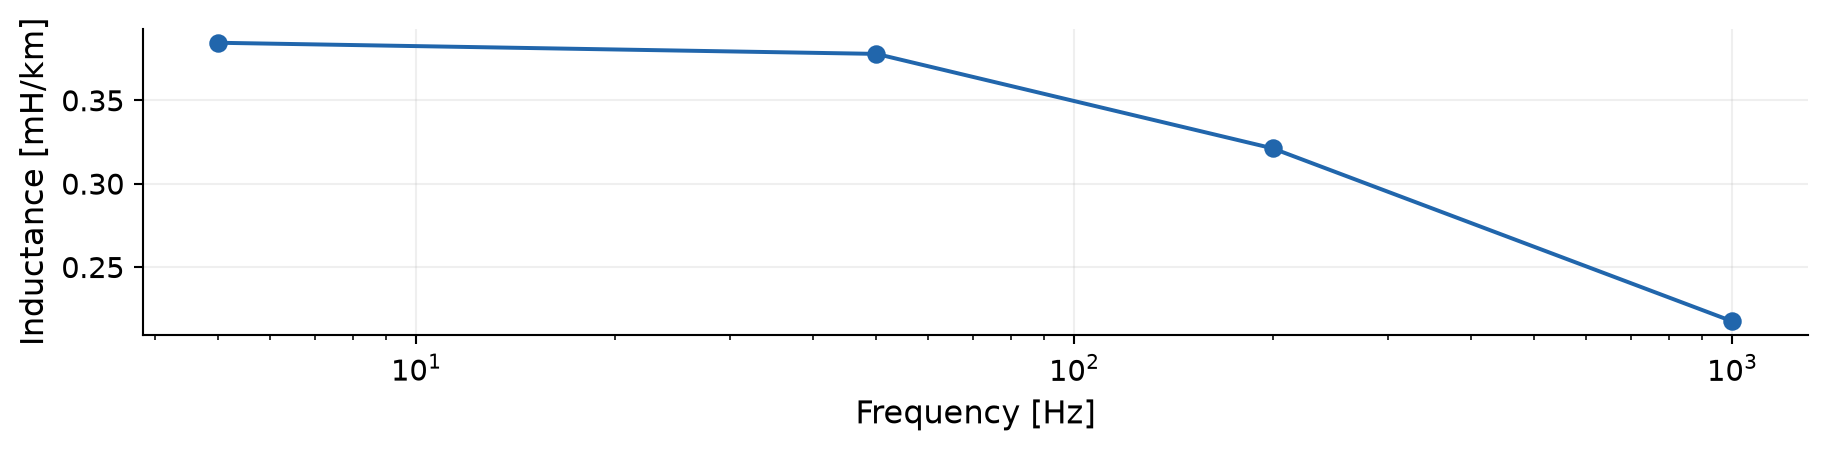
\includegraphics[width=\linewidth,height=2.8cm,keepaspectratio]{figures/frequency.png}\par}
The geometrical external inductance is nearly frequency independent, but skin
effect reduces internal flux penetration and induced screen currents alter the
external field. The effective terminal inductance therefore varies with frequency,
even though all permeabilities are constant.

\newpage
\pagetitle{A change that reduces loss}{Q3.11 --- Single-point screen bonding}
\assignmentquestion{\QuestionThreeEleven}
\guidetitle
\begin{lstlisting}[style=command]
python run.py --case baseline
python run.py --case single_point --single-point --open
\end{lstlisting}
\codeguide
 {Both-end and single-point bonding at the same 415 A RMS and 50 Hz.}
 {\texttt{SinglePoint} in \path{model.pro} changes the screen constraint from
  zero voltage gradient to zero net current. \path{analyse.py} integrates the resulting losses.}
 {Compare \texttt{loss\_screens\_W\_m} and \texttt{loss\_total\_W\_m} in
  \path{results/baseline/metrics.json} and \path{results/single_point/metrics.json}.
  Gmsh opens the single-point field maps; local screen eddy currents remain.}
Replace both-end solid bonding by single-point bonding for each copper screen.
Electrically, one screen end is connected to earth and the other is insulated,
so there is no end-to-end circulating-current loop. In the 2D model this means
\(\widehat I_s=0\), with \(g_s\) solved instead of imposed.

\begin{table}[H]\centering
\caption{Loss reduction at the same 415 A RMS and 50 Hz.}
\begin{tabular}{@{}lrr@{}}\toprule
Quantity & Solid bonding & Single point\\\midrule
Copper loss [kW/km] & \val{\CuLoss} & \val{\SingleCu}\\
Total loss [kW/km] & \val{\BaseLoss} & \val{\SingleLoss}\\\bottomrule\end{tabular}\end{table}
The reduction is \val{\SavingAbsolute} kW/km, or \pct{\Saving} of total MQS
loss. Net screen current disappears while local eddy currents remain, so copper
loss does not become exactly zero. The aluminium loss changes slightly too,
because the screen field and phase current redistribution change together.

\begin{figure}[H]\centering
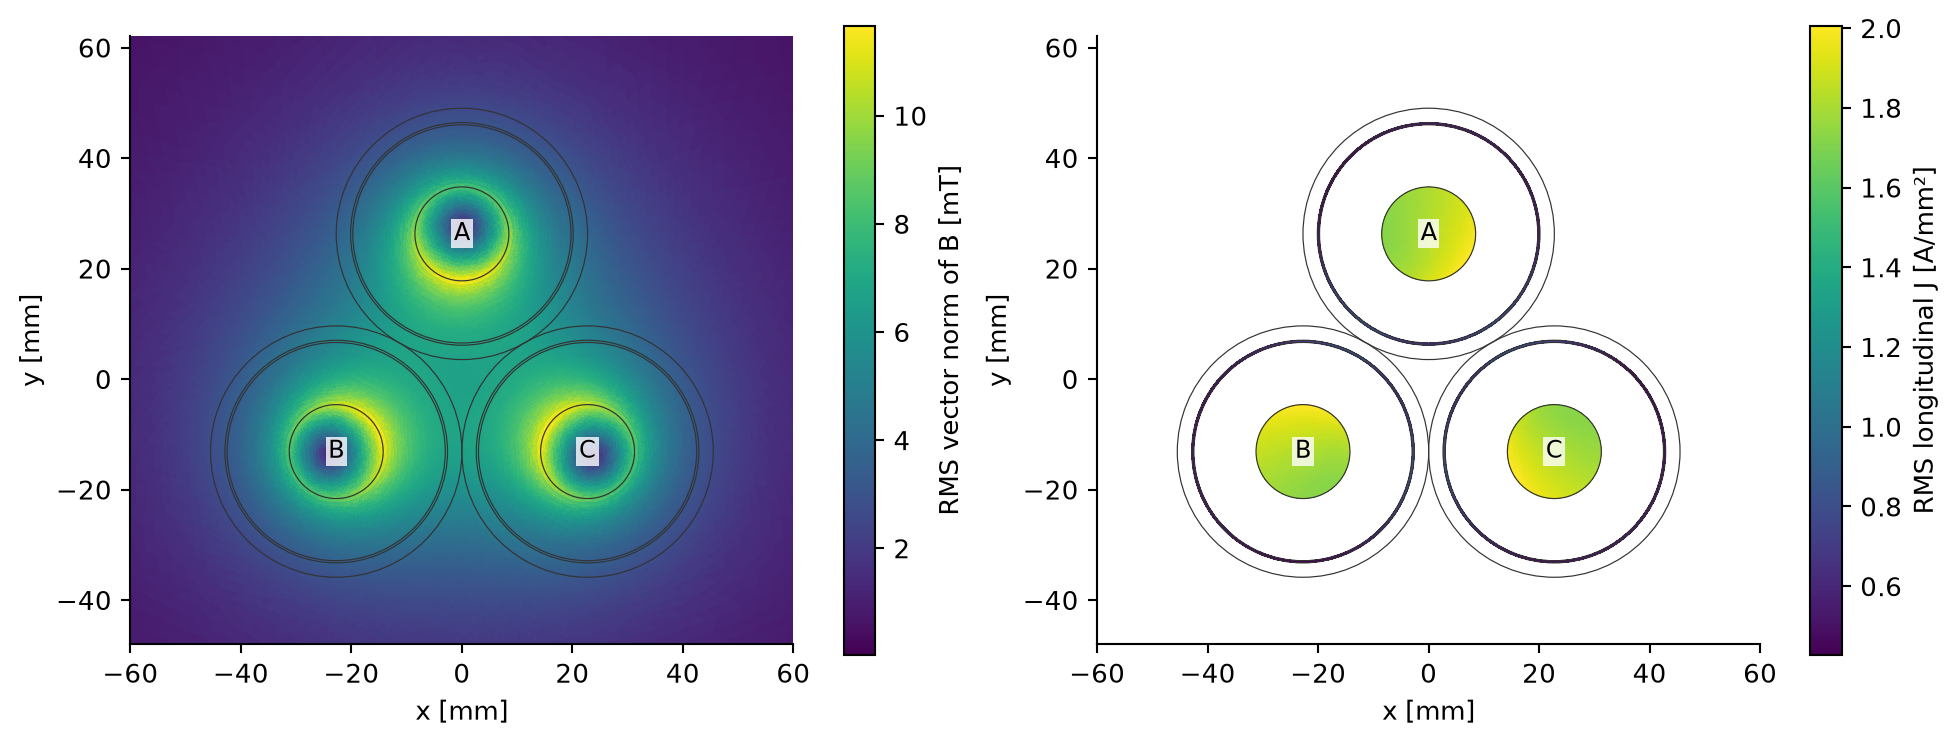
\includegraphics[width=\linewidth,height=5.8cm,keepaspectratio]{figures/single_point_fields.png}
\caption{Single-point bonding retains magnetic penetration and local screen
eddy currents. The improvement comes from suppressing net circulating current.}
\end{figure}

\subhead{What the change establishes}
The result is a quantified loss improvement for the equivalent straight,
isothermal cable model. NKT lists both single-point and both-end bonding;
for the selected 240 \(\mathrm{mm^2}\) directly buried touching-trefoil row,
both are rated 415 A [2]. A loss reduction therefore does not justify replacing
the published rating with a calculated higher ampacity.

Single-point bonding creates a longitudinal screen voltage at the open end.
Its acceptability depends on route length, bonding leads, sheath voltage limiters,
fault conditions and touch-voltage design. The model supplies a voltage gradient,
but the assignment gives no route length from which to calculate an end voltage.
This proposal is consequently a comparison of bonding schemes, with a full
installation design and the coupled thermal calculation still required.

\newpage
\pagetitle{Rebuilding the PDF and sources}{Section 3 --- Numerical record}
\subhead{After completing the study}
With the Python environment activated, run from \path{Source-code/section_3}:
\begin{lstlisting}[style=command]
cd ../..
./LaTeX/build_section_3.sh
\end{lstlisting}
The builder exports the completed study and compiles this report with
\texttt{pdflatex}; it does not rerun the FE cases.
The executed versions are Gmsh 4.15.0-git and GetDP
4.0.0-git-259f4c38 (PETSc real arithmetic). Full build information is stored
under \path{Source-code/section_3/validation/}.
The report exporter checks input hashes against every saved case before
using it. The PDF build uses these verified results and does not silently
solve a different study. Numerical residuals are collected in
\path{Source-code/section_3/validation/RESULTS.md}.

\subhead{References}
\textbf{[1]} R.~V.~Sabariego, \emph{Electromagnetic and thermal analysis of a
high voltage cable}, NMES Assignment 2026, Section 3 and Appendices A--B,
KU Leuven. Local source: \path{NMES_Assignment_2026.pdf}.

\textbf{[2]} NKT, \emph{33 kV single core cable XLPE-AL}, printed pp.~19--20,
240 \(\mathrm{mm^2}\) column. Local source:\par
\texttt{Datasheet 33 kV single core cable XLPE-AL.pdf}.

\textbf{[3]} Supplied TA \path{magnetodynamic_formulation.pro} and
\path{shared/Jacobian_Integration.pro}. The original formulations are preserved;
the cable-specific massive/stranded implementation is in \path{section_3/model.pro}.

\textbf{[4]} GetDP reference manual, function spaces, global quantities and
2D magnetoquasistatic formulations:
\url{https://getdp.info/doc/texinfo/getdp.html}.

\textbf{[5]} Section 1 report, material table and resistance calibration.
Copper conductivity \(5.95\times10^7~\mathrm{S/m}\), effective aluminium
conductivity \(3.52454\times10^7~\mathrm{S/m}\), semiconductor conductivity
\(0.002~\mathrm{S/m}\), and soil conductivity \(0.01~\mathrm{S/m}\) are
inherited from that stated model, with their original provenance.

\end{document}
